\begin{figure}[]
\begin{subfigure}{\textwidth}
  \centering
  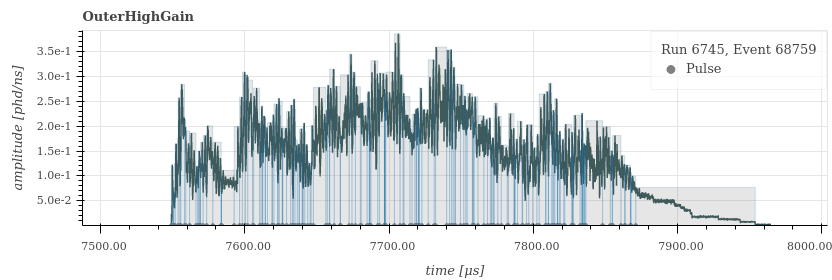
\includegraphics[width=\linewidth]{Figures/OD_Backgrounds/noise_pulse.png}
  \caption{High noise period.}
  \label{fig:noise_od_waveform}
  \end{subfigure}
  \begin{subfigure}{\textwidth}
  \centering
  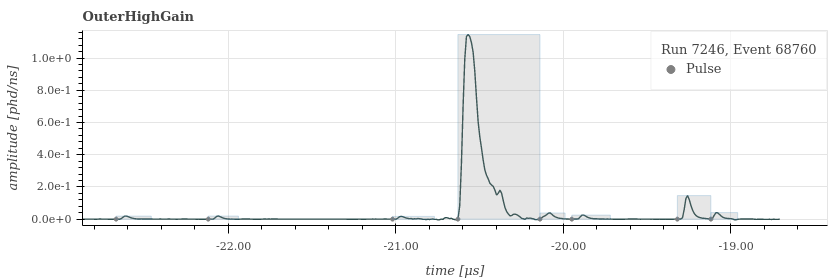
\includegraphics[width=\linewidth]{Figures/OD_Backgrounds/regular_pulse.png}
  \caption{Regular pulses}
  \label{fig:regular_od_waveform}
  \end{subfigure}
\caption{OD summed waveforms showing a noisy period and a regular time.}
\label{fig:od_noise_cut_waveforms}
\end{figure}


\begin{figure}[]%
\centering
\begin{tikzpicture}
\centering
  \begin{axis}[%point meta max=150,
    %point meta min=0.0,
    height=10cm, width=10cm,
    view={0}{90},
    ylabel={Pulse Amplitude/Pulse Area},
    xlabel={Pulse Area (phd)},
    xmin=0, ymin=0,
    colorbar,
    colorbar style={ylabel={Count},ymode=log,},
    ]
    \addplot3[
      surf,
      shader=flat corner,
	  mesh/cols=22,
	  mesh/ordering=rowwise,
	  point meta = {z<0.1 ? nan : z}
    ] file {Data/OD_Energy_Scale/noise_cut_2d_low.dat};
    
    \addplot3[
      surf,
      shader=flat corner,
	  mesh/cols=30,
	  mesh/ordering=rowwise,
	  point meta = {z<0.1 ? nan : z}
    ] file {Data/OD_Energy_Scale/noise_cut_2d_high.dat};
\end{axis}
\end{tikzpicture}
\caption{Representative pulses seen in the OD during SR1.
         No pulse selection has been applied.
         Real events are in the distribution around 0.01 height/area.}
\label{fig:od_noise_cut}
\end{figure}